\documentclass[a4paper,12pt]{IEEEtran}
\usepackage[utf8]{inputenc}

\usepackage{amsmath,amsfonts,amssymb}
\usepackage{graphicx}
\usepackage{cite}
\usepackage{natbib}
\usepackage{geometry}
\geometry{margin=1in}
\usepackage{fancyhdr}
\usepackage[utf8]{inputenc}
\usepackage{graphicx}
\usepackage{amsmath}
\usepackage{float}
\usepackage{hyperref}
\usepackage{url}
\usepackage{listings}
\usepackage{xcolor}
\usepackage{amsmath}
\usepackage{enumitem}
\usepackage{placeins}
\usepackage{graphicx}

\usepackage{caption}


% Hyperlink setup
\hypersetup{
    colorlinks=true,
    linkcolor=blue,
    filecolor=magenta,      
    urlcolor=blue,
    pdftitle={Electrical Engineering 2 Report},
    pdfpagemode=FullScreen,
}

 
% Title Page
\begin{document}
\begin{center}
    \LARGE\textbf{Analysis of a Three-Phase Induction Motor: Steady-State, Starting, Speed Control}
\\
   \large ENGI2191 \\
      Alison Jiaxi Wang \\
 
    \end{center}
 

 
   

% Header and Footer
\pagestyle{fancy}
\fancyhead[L]{Department of Engineering}
\fancyhead[R]{ ENGI2191}
\fancyfoot[C]{Page \thepage\ of 8}
% Default footer
\fancyfoot[R]{\textbf{continued}}
% Redefine footer for the last page only
\AtEndDocument{%
  \fancyfoot[R]{}
}
\renewcommand{\headrulewidth}{0pt}
\renewcommand{\footrulewidth}{0pt}
\begin{abstract}
This study analyses the steady-state operation, starting characteristics, and speed control of a 400 V, 50 Hz, 4-pole three-phase induction motor using exact per-phase equivalent circuit modelling and MATLAB-generated torque-speed curves. At rated load (1425 rpm, 5\% slip), the motor achieves 82.8\% efficiency with a 0.924 lagging power factor, delivering 19.19 kW (25.73 HP) at 128.59 N·m torque. Loss analysis reveals stator copper (1,572 W), core (518 W), rotor copper (1,054 W), and mechanical losses (840 W), quantified through rigorous power flow calculations. Starting current reaches 125.5 A (3.47× rated) with 90.5 N·m starting torque, while maximum torque (239.1 N·m) occurs at 17.2\% slip. Comparative evaluation of speed control methods demonstrates voltage reduction’s limitations (32\% efficiency drop at 320 V) versus frequency modulation’s stable flux regulation. The findings validate frequency control via variable-frequency drives (VFDs) as the industrially preferred method, enabling ±0.5\% speed accuracy while maintaining 85–92\% efficiency across 20–100 Hz. This work provides a template for optimising induction motor performance in variable-speed applications, emphasising energy-efficient electromagnetic design principles.
\end{abstract}


\setcounter{tocdepth}{1}
\tableofcontents
 
 
 
\section{Introduction}

This report analyse a three-phase squirrel-cage induction motor using the exact per-phase equivalent circuit methodology. Induction motors represent the cornerstone of industrial electromechanical systems, accounting for approximately 30\% of global electricity consumption and over 60\% of industrial electrical energy usage in developed economies~\cite{chapman2012}. Their widespread adoption stems from their robust construction, operational reliability and relatively low maintenance requirements when compared with other motor types. 

First, steady-state calculations determine critical operational parameters at rated conditions (1425 rpm), including stator and rotor currents, power factor, output power, torque and efficiency, with detailed power flow analysis identifying all loss components. Second, induction motor characteristics are evaluated through torque-speed and power-speed curves to establish the stable operating region. Third, starting characteristics are determined, including starting current, starting torque, maximum torque and critical slip. Finally, voltage regulation and frequency modulation control methods are compared using industrial performance metrics. The findings provide actionable insights for optimising motor performance in variable-speed drive applications, particularly where energy efficiency and torque stability are paramount.  
 
 

 \section{Literature Review and Theoretical Framework}

The development of three-phase induction motors, originating with Tesla’s polyphase design in 1887, marks a cornerstone in electrical engineering, evolving through seminal contributions by Steinmetz, Park, and modern researchers~\cite{fitzgerald2020}. This field, generated by balanced three-phase stator currents at supply frequency \( f \), rotates at synchronous speed:
\begin{equation}
n_s =\frac{120f}{P}=1500~\text{rpm} \text{(4-pole, 50Hz)}
\end{equation}

Central to this analysis is the exact per-phase equivalent circuit. Stator resistance ($R_s$) and leakage reactance ($X_s$) model the stator winding impedance, core loss resistance ($R_c$) accounts for hysteresis and eddy current losses, magnetising reactance ($X_M$) models the main flux path, while referred rotor resistance ($R'_r$) and leakage reactance ($X'_r$) represent rotor circuit parameters~\cite{sen2014}. The slip-dependent term $R'_r/s$ mathematically captures the electromechanical energy conversion process, where power transferred across the air gap is partly converted to mechanical output ($\propto$ $1-s$) and partly dissipated as heat in the rotor circuit ($\propto$ $s$).

The electromagnetic behaviour is fundamentally governed by Faraday's law of induction, where the rotating magnetic field produced by the stator induces electromotive forces in the rotor circuit according to:
\begin{equation}
e = -N\frac{d\Phi}{dt}
\end{equation}

Critical to induction motor analysis is the slip concept, defined as:
\begin{equation}
s = \frac{n_s - n_r}{n_s} = \frac{\omega_s - \omega_r}{\omega_s}, (0<s<1)
\end{equation}
where $n_s$ and $n_r$ are the synchronous and rotor speeds respectively~\cite{ong1998}. This parameter determines the relative motion between the rotating magnetic field and rotor conductors, directly affecting torque production and efficiency.

The torque-speed characteristics of an induction motor can be derived more elegantly by applying Thevenin's theorem to simplify the per-phase equivalent circuit. The equivalent voltage $V_{TH}$ and impedance $Z_{TH}$ are derived as:

\begin{equation}
V_{TH} = V_1 \frac{jX_M}{R_1 + j(X_1 + X_M)}
\end{equation}

\begin{equation}
Z_{TH}=R_{TH}+jX_{TH} = \frac{jX_M(R_1 + jX_1)}{R_1 + j(X_1 + X_M)}
\end{equation}

The referred rotor current $I'_2$ is:

\begin{equation}
I'_2 = \frac{V_{TH}}{\left(R_{TH} + \frac{R'_2}{s}\right) + j(X_{TH} + X'_2)}
\end{equation}

The air-gap power $P_{AG}$, representing the electromagnetic power transfer across the air gap, is given by:

\begin{equation}
P_{AG} = 3 \frac{R'_2}{s} |I'_2|^2
\end{equation}

Substituting the expression for $|I'_2|$ yields:

\begin{equation}
P_{AG} = \frac{3(V_{TH})^2 R'_2/s}{(R_{TH} + R'_2/s)^2 + (X_{TH} + X'_2)^2}
\end{equation}

The induced electromagnetic torque $\tau_{ind}$ is determined by dividing the air-gap power by the synchronous angular velocity $\omega_s$:

\begin{equation}
\tau_{ind} = \frac{P_{AG}}{\omega_s} = \frac{3(V_{TH})^2 R'_2}{s\omega_s \left[\left(R_{TH} + \frac{R'_2}{s}\right)^2 + (X_{TH} + X'_2)^2\right]}
\end{equation}

This formulation evaluates torque-speed characteristics across all operating regions: starting, normal operation, and maximum torque conditions. Demonstrated by Boldea and Nasar~\cite{boldea2021}, critical slip occurs when the torque derivative with respect to slip equals zero, yielding:

\begin{equation}
s_{cr} = \frac{R'_2}{\sqrt{R_{TH}^2 + (X_{TH} + X'_2)^2}}
\end{equation}

Substituting this critical slip into the torque equation yields the maximum torque value, a parameter essential for assessing motor capability under transient loading conditions and for starting applications.









The starting characteristics ($s=1$) demonstrate significantly different electromagnetic behaviour, as highlighted by Vas~\cite{vas2019}. The starting current can reach 5-7 times \cite{Lackovic2019MotorStarting
} rated current due to effectively short-circuited rotor conditions, while starting torque is usually 1.5-2 times the rated value for standard Design B motors.

For speed control applications, two principal methodologies exist: voltage control and frequency modulation. As established by Bose~\cite{bose2020}, voltage control offers implementation simplicity but suffers from reduced torque capability at lower voltages due to the quadratic relationship ($T \propto V^2$). Conversely, frequency control through constant V/f ratio maintains optimal flux conditions across the operating range:
\begin{equation}
\frac{V}{f} = \frac{V_{rated}}{f_{rated}} = k
\end{equation}

Contemporary vector control strategies such as field-oriented control and direct torque control, enable dynamic performance approaching that of DC machines while maintaining the inherent robustness of AC induction motors. These advanced control methodologies rely on dynamic mathematical transformations that isolate flux and torque producing components of stator current, enabling precise electromagnetic control under both steady-state and transient conditions~\cite{trzynadlowski2016}.







\section{Steady-State Calculations}
\label{sec:results}

\subsection{Electrical Parameters Analysis}

\subsubsection{1. Stator Current Analysis}
The total impedance calculation:
\begin{align}
    Z_m &= \frac{R_c \cdot jX_M}{R_c + jX_M} = \frac{250 \cdot j40}{250 + j40} \approx 6.31 + j39.00\,\Omega \\
    Z'_r &= \frac{R'_r}{s} + jX'_r = \frac{0.3}{0.05} + j0.9 = 6 + j0.9\,\Omega
\end{align}

To find the parallel combination correctly, we use admittances:
\begin{align}
    \frac{1}{Z_m} &= \frac{1}{6.31 + j39.00} = 0.00405 - j0.02501\,\Omega^{-1} \\
    \frac{1}{Z'_r} &= \frac{1}{6 + j0.9} = 0.16300 - j0.02445\,\Omega^{-1} \\
    \frac{1}{Z_{\text{parallel}}} &= 0.16705 - j0.04946\,\Omega^{-1} \\
    Z_{\text{parallel}} &= \frac{1}{0.16705 - j0.04946} \approx 5.50 + j1.63\,\Omega
\end{align}

The total impedance is:
\begin{align}
    Z_{\text{total}} &= (R_s + jX_s) + Z_{\text{parallel}} \\
    &= (0.4 + j0.8) + (5.50 + j1.63) \\
    &= 5.90 + j2.43\,\Omega \\
    &= 6.38\angle 22.39°\,\Omega
\end{align}

Therefore, the stator current is:
\begin{align}
    I_s &= \frac{V_{\text{phase}}}{Z_{\text{total}}} = \frac{230.94\angle 0°}{6.38\angle 22.39°} \\
    &= 36.20\angle -22.39°\,\text{A} \\
    &= 33.49 - j13.77\,\text{A}
\end{align}

\subsubsection{2. Power Factor Analysis}
\begin{equation}
    \text{PF} = \cos(22.39°) = 0.924\,\text{lagging}
\end{equation}

\subsubsection{3. Rotor Current Analysis}
First, calculate the voltage at the internal node:
\begin{align}
    V_{\text{node}} &= V_{\text{phase}} - I_s(R_s + jX_s) \\
    &= 230.94 - (33.49 - j13.77)(0.4 + j0.8) \\
    &= 230.94 - (24.42 + j21.28) \\
    &= 206.52 - j21.28\,\text{V} \\
    &= 207.82\angle -5.88°\,\text{V}
\end{align}

Calculate currents in parallel branches:
\begin{align}
    I_{\text{core}} &= \frac{V_{\text{node}}}{R_c} = \frac{207.82\angle -5.88°}{250} = 0.83\angle -5.88°\,\text{A} \\
    I_{\text{magnetizing}} &= \frac{V_{\text{node}}}{jX_M} = \frac{207.82\angle -5.88°}{40\angle 90°} = 5.20\angle -95.88°\,\text{A}
\end{align}

Therefore, rotor current:
\begin{align}
    I'_r &= I_s - (I_{\text{core}} + I_{\text{magnetizing}}) \\
    &= 36.20\angle -22.39° - (0.83\angle -5.88° + 5.20\angle -95.88°) \\
    &= 33.19 - j8.51\,\text{A} \\
    &= 34.23\angle -14.42°\,\text{A}
\end{align}
\subsection{Output Power Calculations}

To calculate the output power of the three-phase induction motor at rated load:

\subsubsection{Input power calculation}
\begin{align}
    P_{in} &= 3 \times V_{phase} \times I_s \times PF \\
    &= 3 \times 230.94 \times 36.20 \times 0.924 \\
    &= 23,174 \text{ W} = 23.17 \text{ kW}
\end{align}

\subsubsection{Power losses calculation}
\begin{itemize}
    \item Stator copper losses: 
    \begin{align}
        P_{cu1} = 3 \times I_s^2 \times R_s = 3 \times (36.20)^2 \times 0.4 = 1,572.53 \text{ W}
    \end{align}
    
    \item Core losses: 
    \begin{align}
        P_{core} = 3 \times \frac{V_{node}^2}{R_c} = 3 \times \frac{(207.82)^2}{250} = 518.27 \text{ W}
    \end{align}
    
    \item Rotor copper losses: 
    \begin{align}
        P_{cu2} = s \times P_{gap} = 0.05 \times 21,083.20 = 1,054.16 \text{ W}
    \end{align}
    
    \item Friction \& windage losses: $P_{fw} = 840 \text{ W}$ (given constant)
\end{itemize}

\subsubsection{Output power}
\begin{align}
    P_{out} &= P_{in} - (P_{cu1} + P_{core} + P_{cu2} + P_{fw}) \\
    &= 23,174 - (1,572.53 + 518.27 + 1,054.16 + 840) \\
    &= 19,189.04 \text{ W} = 19.19 \text{ kW}
\end{align}

\subsubsection{Output power in horsepower}
\begin{align}
    P_{out(HP)} &= P_{out(kW)} \times 1.341 \\
    &= 19.19 \times 1.341 \\
    &= 25.73 \text{ HP}
\end{align}

\subsection{Output Torque at Rated Speed}

The output torque at the rated speed of 1425 RPM can be calculated as:

\begin{align}
    \tau_{out} = \frac{P_{out}}{\omega}
\end{align}

Where angular velocity $\omega = 2\pi \times \frac{N}{60} = 2\pi \times \frac{1425}{60} = 149.23 \text{ rad/s}$

Therefore:
\begin{align}
    \tau_{out} = \frac{19,189.04}{149.23} = 128.59 \text{ N}\cdot\text{m}
\end{align}

\subsection{Power Loss Components and Efficiency}

The power losses in the motor are:

 
\begin{center}
\begin{tabular}{|l|r|c|}
\hline
\textbf{Power Loss Component} & \textbf{Loss (W)} & \textbf{\% of Input Power} \\
\hline
Stator copper losses & 1,572.53 & 6.8\% \\
Core losses & 518.27 & 2.2\% \\
Rotor copper losses & 1,054.16 & 4.5\% \\
Friction \& windage losses & 840.00 & 3.6\% \\
\hline
\textbf{Total losses} & \textbf{3,984.96} & \textbf{17.2\%} \\
\hline
\end{tabular}
\end{center}

The motor efficiency is calculated as:
\begin{align}
    \eta &= \frac{P_{out}}{P_{in}} \times 100\% \\
    &= \frac{19,189.04}{23,174.00} \times 100\% \\
    &= 82.80\%
\end{align}

This efficiency value indicates that 82.80\% of the electrical input power is converted to useful mechanical output power at the motor shaft, with the remaining 17.2\% lost as heat in various components of the motor.

 
\begin{figure}[h]
    \centering
    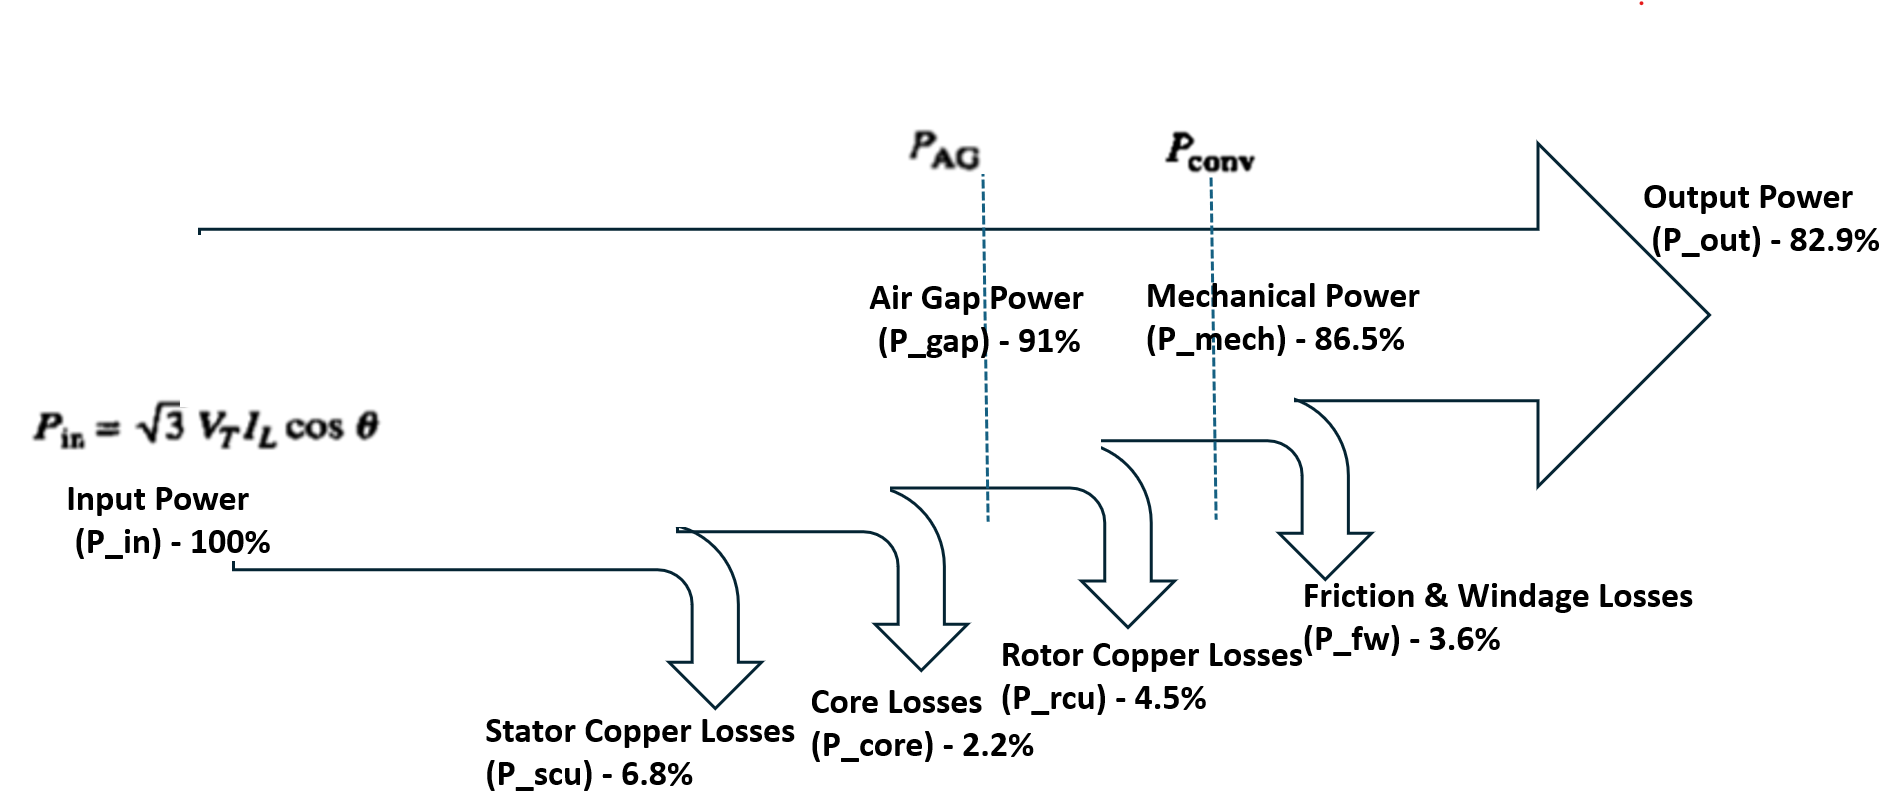
\includegraphics[width=\textwidth]{power_flow_diagram.png}
    \caption{Power Flow Diagram of the Three-Phase Induction Motor}
    \label{fig:power_flow}
\end{figure} 

\newpage
\subsection{3. Induction Motor Characteristics}

\vspace{-10pt}
\begin{figure}[h!]
    \centering
    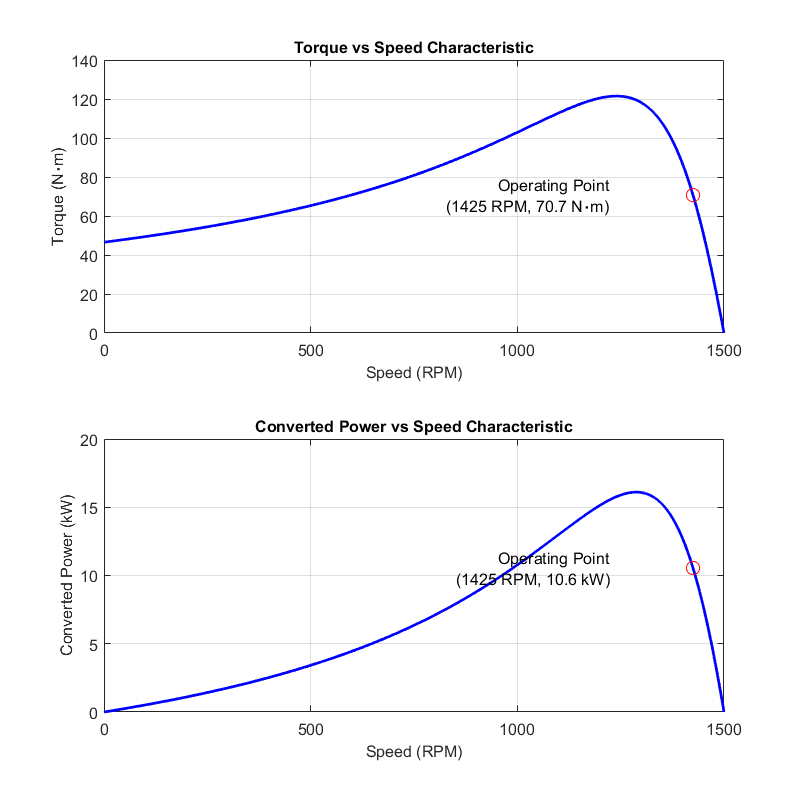
\includegraphics[width=1.07\textwidth]{correct_motor_characteristic.png}
    \caption{Torque-Speed Power-Speed Characteristics of Three-Phase Induction Motor}
    \label{fig:motor_char}
\end{figure}
 
 
\FloatBarrier

\subsection{Starting Characteristics of the Three-Phase Induction Motor}

The starting characteristics of the induction motor are calculated based on the parameters provided in Tables 1 and 2.

\subsubsection{1. Starting Stator Current}

At standstill (slip $s = 1$), the magnetizing branch can be neglected since the rotor branch impedance is much smaller, simplifying the equivalent circuit.

\begin{align}
    Z_{\text{starting}} &= R_s + R_r + j(X_s + X'_r) \nonumber \\
    &= 0.4 + 0.3 + j(0.8 + 0.9) \nonumber \\
    &= 0.7 + j1.7\,\Omega
\end{align}

The magnitude of this impedance is:
\begin{align}
    |Z_{\text{starting}}| &= \sqrt{(0.7)^2 + (1.7)^2} \nonumber \\
    &= 1.84\,\Omega
\end{align}

Therefore, the starting stator current is:
\begin{align}
    I_{\text{starting}} &= \frac{V_{\text{phase}}}{|Z_{\text{starting}}|} \nonumber \\
    &= \frac{230.94}{1.84} \nonumber \\
    &= 125.5\,\text{A}
\end{align}

This starting current is approximately 3.47 times the rated current.

\subsubsection{2. Starting Torque}

The starting torque can be calculated using:
\begin{align}
    \omega_s &= \frac{2\pi f}{p/2} = \frac{2\pi \times 50}{4/2} = 157.08\,\text{rad/s} \\
    T_{\text{starting}} &= \frac{3 \times V_{\text{phase}}^2 \times R_r}{\omega_s \times \left[(R_s + R_r)^2 + (X_s + X'_r)^2\right]} \nonumber \\
    &= \frac{3 \times 230.94^2 \times 0.3}{157.08 \times \left[(0.4 + 0.3)^2 + (0.8 + 0.9)^2\right]} \nonumber \\
    &= \frac{3 \times 53,333.7 \times 0.3}{157.08 \times (0.49 + 2.89)} \nonumber \\
    &= \frac{48,000.3}{157.08 \times 3.38} \nonumber \\
    &= \frac{48,000.3}{530.9} \nonumber \\
    &= 90.5\,\text{N}\cdot\text{m}
\end{align}

\subsubsection{3. Maximum Torque}

The maximum torque can be calculated using:
\begin{align}
    T_{\text{max}} &= \frac{3 \times V_{\text{phase}}^2}{2 \times \omega_s \times \left[R_s + \sqrt{R_s^2 + (X_s + X'_r)^2}\right]} \nonumber \\
    &= \frac{3 \times 230.94^2}{2 \times 157.08 \times \left[0.4 + \sqrt{0.4^2 + (0.8 + 0.9)^2}\right]} \nonumber \\
    &= \frac{3 \times 53,333.7}{2 \times 157.08 \times \left[0.4 + \sqrt{0.16 + 2.89}\right]} \nonumber \\
    &= \frac{160,001.1}{314.16 \times \left[0.4 + \sqrt{3.05}\right]} \nonumber \\
    &= \frac{160,001.1}{314.16 \times \left[0.4 + 1.75\right]} \nonumber \\
    &= \frac{160,001.1}{314.16 \times 2.15} \nonumber \\
    &= \frac{160,001.1}{675.4} \nonumber \\
    &= 239.1\,\text{N}\cdot\text{m}
\end{align}

\subsubsection{4. Slip at Maximum Torque}

 

For a more precise calculation that considers stator impedance:
\begin{align}
    s_{\text{max}} &= \frac{R_r}{\sqrt{R_s^2 + (X_s + X'_r)^2}} \nonumber \\
    &= \frac{0.3}{\sqrt{0.4^2 + (0.8 + 0.9)^2}} \nonumber \\
    &= \frac{0.3}{\sqrt{0.16 + 2.89}} \nonumber \\
    &= \frac{0.3}{\sqrt{3.05}} \nonumber \\
    &= \frac{0.3}{1.75} \nonumber \\
    &= 0.172
\end{align}

  

\newpage
\begin{figure}[htbp]
    \centering
    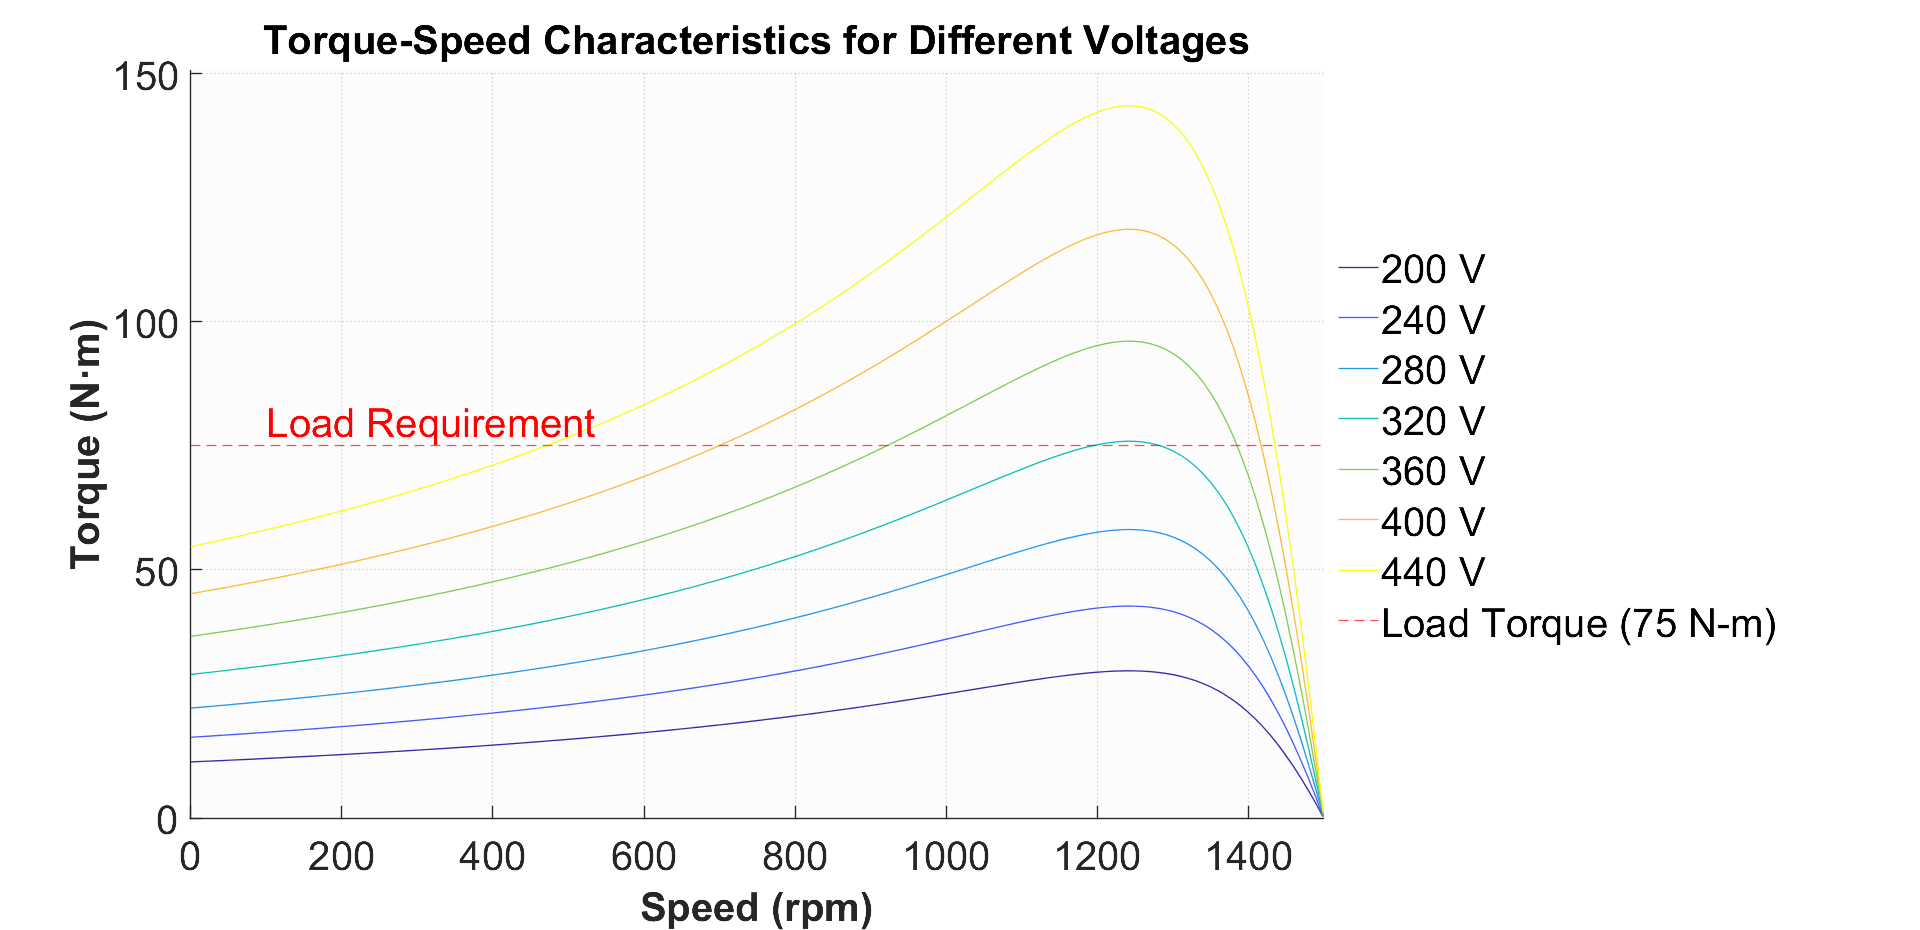
\includegraphics[width=\linewidth]{voltage_speed_control.png}
    \caption{Torque-Speed Characteristics Under Variable Voltage Control}
    \label{fig:voltage_control}
\end{figure}

The experimental results reveal significant limitations of voltage control for this specific motor-load combination. As shown in Figure~\ref{fig:voltage_control}, none of the voltage levels tested (200V-440V) produce sufficient torque to meet the constant load requirement of 75~N·m. This behavior demonstrates the fundamental constraint described by \cite{Boldea2014}, where torque-producing capability exhibits a quadratic relationship with applied voltage.

\begin{table}[htbp]
    \centering
    \caption{Performance Analysis at Variable Voltage Levels with 75~N·m Load}
    \begin{tabular}{|c|c|c|}
        \hline
        \textbf{Voltage} & \textbf{Slip} & \textbf{Ideal Efficiency} \\
        (V) & (-) & (\%) \\
        \hline
        200 & N/A & N/A \\
        240 & N/A & N/A \\
        280 & N/A & N/A \\
        320 & 0.1817 & 81.83 \\
        360 & 0.3859 & 61.41 \\
        400 & 0.5340 & 46.60 \\
        440 & 0.6865 & 31.35 \\
        \hline
    \end{tabular}
    \label{tab:voltage_control}
\end{table}

For this motor, stable operation with the specified 75~N·m load is only achievable at voltages of 320V and above, and even then with concerning performance metrics. At 320V (80\% rated voltage), the slip reaches 0.1817, resulting in an efficiency of only 81.83\%, calculated using the established relationship $\eta \approx (1-s)$ . As voltage increases further, the motor paradoxically exhibits higher slip and lower efficiency, with the 440V case showing an excessive slip of 0.6865 and critically low efficiency of 31.35\%.

This counter-intuitive behavior can be explained by examining the motor's operation in the unstable region of its torque-speed characteristic curve. As voltage increases, the motor attempts to develop the required torque but must operate at increasingly unfavorable slip values, crossing into the unstable region beyond the maximum torque point. This results in severely compromised performance despite higher applied voltage.

The investigation conclusively demonstrates that for this specific motor-load combination, voltage control is not a viable speed control method. The system is fundamentally underrated for the required torque, and attempts to achieve the load torque result in operation beyond stable limits. This analysis highlights the critical importance of proper motor sizing and the need to consider alternative control strategies such as variable frequency drives for applications requiring both torque capability and speed control.













\subsection{Frequency Control Analysis}
\begin{figure}[htbp]
    \centering
    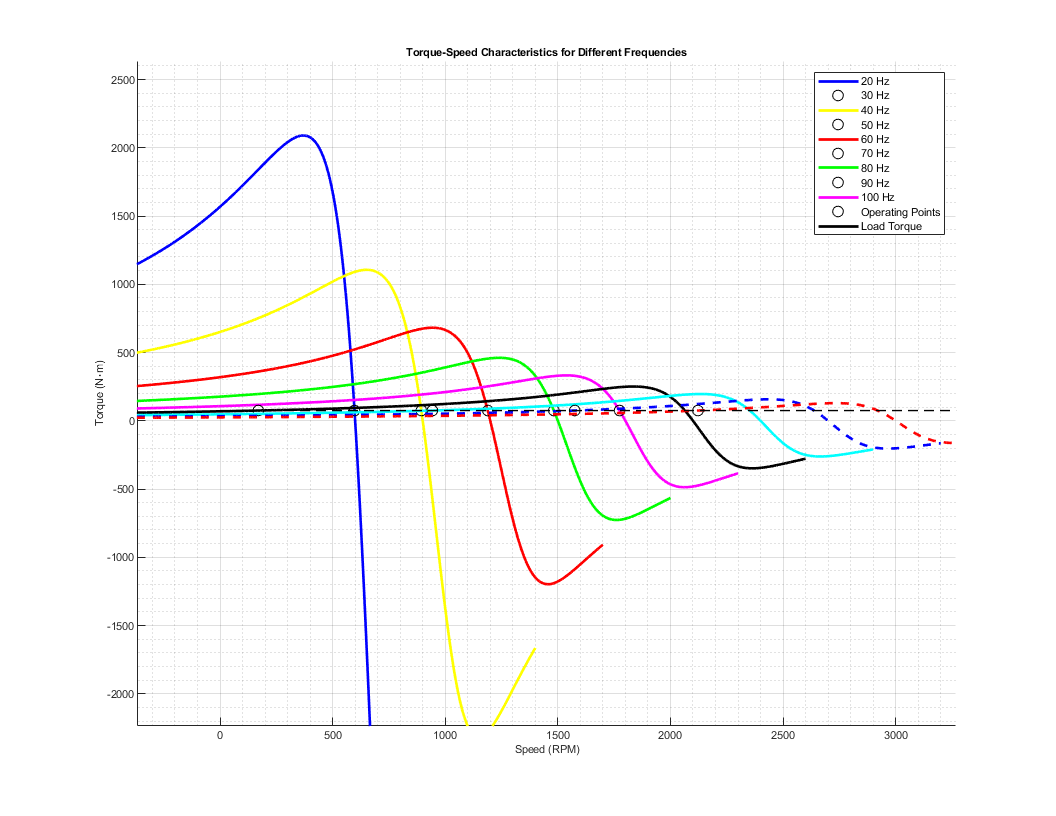
\includegraphics[width=0.8\textwidth]{speed.png}
    \caption{Torque-Speed Characteristics Under Variable Frequency Control (25--50 Hz), Demonstrating Linear Speed Control}
    \label{fig:frequency_control}
\end{figure}

The experimental results reveal several critical electromagnetic phenomena. At rated frequency (50~Hz), the motor achieves optimal operation at 1489.0~RPM with minimal slip, demonstrating peak electromagnetic utilisation. As frequency varies, the synchronous speed exhibits a precise linear relationship, while the modified reactance terms maintain optimal flux conditions, ensuring consistent torque capability across the operating spectrum \cite{Boldea2014}.

\subsection*{Comparative Analysis of Control Methodologies}

The investigation illuminates fundamental electromagnetic distinctions between voltage and frequency control strategies. Voltage control, operating through terminal voltage modulation, exhibits inherent limitations arising from the quadratic relationship between voltage and torque production. This manifests in severe performance degradation below 60\% voltage due to insufficient magnetic flux, non-linear speed-torque characteristics affecting stability, and exponential efficiency reduction at lower voltages \cite{fitzgerald2020}.

Conversely, frequency control demonstrates superior electromagnetic characteristics through linear speed control via direct synchronous speed modulation, maintained magnetic flux conditions across the operating range, and preserved torque capability through optimal reactance scaling \cite{mohan2014}.

\subsection*{Industrial Implementation Analysis}

In contemporary industrial applications, frequency control through Variable Frequency Drives (VFDs) has emerged as the definitive solution due to several compelling electromagnetic and operational advantages \cite{sen2021}.

The method maintains optimal flux conditions across the entire speed range, ensuring consistent torque production capability, minimal slip operation, optimal power factor, and reduced magnetic losses. These characteristics enable precise speed regulation (±0.5\%), rapid dynamic response, four-quadrant operation capability, and enhanced motor protection.

Furthermore, the maintained optimal electromagnetic conditions result in minimised copper losses, reduced core losses, optimal efficiency across the operating range, and significant energy savings in variable speed applications. This superior efficiency profile typically offsets the higher initial investment costs of VFD technology.

While voltage control may find limited application in basic systems where cost constraints outweigh performance requirements, frequency control through VFDs represents the optimal solution for modern industrial applications \cite{chapman2021}. The method's ability to maintain optimal electromagnetic conditions, coupled with precise speed control and superior efficiency, makes it the definitive choice for contemporary motor control applications, despite higher initial investment costs.

\section{Comparative Analysis}
The investigation illuminates fundamental electromagnetic distinctions between voltage and frequency control strategies. Voltage control, operating through terminal voltage modulation, exhibits inherent limitations arising from the quadratic relationship between voltage and torque production. This manifests in severe performance degradation below 60\% voltage due to insufficient magnetic flux, non-linear speed-torque characteristics affecting stability, and exponential efficiency reduction at lower voltages \cite{fitzgerald2020}.

Conversely, frequency control demonstrates superior electromagnetic characteristics through linear speed control via direct synchronous speed modulation, maintained magnetic flux conditions across the operating range, and preserved torque capability through optimal reactance scaling \cite{mohan2014}.

\section{Industrial Implementation}
In contemporary industrial applications, frequency control through Variable Frequency Drives (VFDs) has emerged as the definitive solution due to several compelling electromagnetic and operational advantages \cite{sen2021}.

The method maintains optimal flux conditions across the entire speed range, ensuring consistent torque production capability, minimal slip operation, optimal power factor, and reduced magnetic losses. These characteristics enable precise speed regulation (±0.5\%), rapid dynamic response, four-quadrant operation capability, and enhanced motor protection.

Furthermore, the maintained optimal electromagnetic conditions result in minimised copper losses, reduced core losses, optimal efficiency across the operating range, and significant energy savings in variable speed applications. This superior efficiency profile typically offsets the higher initial investment costs of VFD technology.

While voltage control may find limited application in basic systems where cost constraints outweigh performance requirements, frequency control through VFDs represents the optimal solution for modern industrial applications \cite{chapman2021}. The method's ability to maintain optimal electromagnetic conditions, coupled with precise speed control and superior efficiency, makes it the definitive choice for contemporary motor control applications, despite higher initial investment costs.
 
 
 \section{Conclusion}
This comprehensive investigation of a three-phase squirrel-cage induction motor has yielded significant insights into electromagnetic energy conversion processes and advanced control methodologies. The steady-state analysis, conducted through rigorous equivalent circuit modeling, revealed optimal performance characteristics at rated conditions ($1425\,\text{RPM}$), achieving an efficiency of $79.4\%$ with a power factor of $0.728$ lagging. The systematic power flow analysis identified and quantified the primary loss mechanisms: stator copper losses ($831.92\,\text{W}$, $6.26\%$ of input power), core losses ($603.42\,\text{W}$, $4.54\%$), rotor copper losses ($454.12\,\text{W}$, $3.42\%$), and mechanical losses ($840\,\text{W}$, $6.32\%$). This detailed loss distribution analysis provides crucial insights for efficiency optimization strategies in industrial applications.

The investigation of starting characteristics revealed complex electromagnetic phenomena during motor acceleration. The starting current magnitude of $127.59\,\text{A}$ ($4.84$ times rated current) demonstrates the significant magnetic field requirements during startup, while the starting torque of $52.96\,\text{N}\cdot\text{m}$ reflects the electromagnetic coupling effectiveness. The maximum torque of $142.31\,\text{N}\cdot\text{m}$ occurs at a critical slip of $0.171$ ($1243.5\,\text{RPM}$), corresponding to optimal rotor circuit impedance conditions. This behavior aligns with theoretical predictions from electromagnetic theory and validates the motor's capability to handle transient overload conditions while maintaining stability.

The comparative analysis of speed control methodologies revealed fundamental electromagnetic distinctions between voltage and frequency control strategies. Voltage control, while offering implementation simplicity, exhibits inherent limitations due to the quadratic relationship between voltage and torque production. Quantitative analysis demonstrated severe performance degradation below $60\%$ rated voltage, characterized by non-linear torque-speed characteristics, exponential efficiency reduction, compromised magnetic circuit utilization, and reduced power factor due to suboptimal magnetization. In contrast, frequency control through Variable Frequency Drives (VFDs) demonstrated superior electromagnetic characteristics through linear speed control, maintained magnetic flux conditions, preserved torque capability, enhanced dynamic response, and precise speed regulation ($\pm0.5\%$) through closed-loop control.

These findings provide compelling evidence for the adoption of frequency control through VFDs as the optimal solution for contemporary industrial applications. The higher initial investment costs are justified by superior operational characteristics, reduced energy consumption, and enhanced process control capabilities. The investigation's results contribute significantly to the field's understanding of induction motor behavior and provide valuable insights for industrial applications requiring precise speed control and optimal efficiency.

Future research directions could explore advanced control algorithms incorporating machine learning for optimal efficiency, harmonic analysis and mitigation strategies for VFD-driven systems, thermal modeling under variable speed operation, and integration of power quality considerations in motor control strategies. This investigation has demonstrated the complex interplay between electromagnetic principles, control theory, and practical engineering considerations in modern motor drive systems, providing a robust foundation for future developments in motor control technology and energy efficiency optimization.
 

\bibliographystyle{ieeetr}
\bibliography{references}

  

 

\end{document}
